\subsection{Initial testing}\label{sec:initialtest}
In this section several tests will be performed which does not require the cluster. These tests will be run to find the settings the cluster should be run with when the final cluster tests will be performed.

\subsubsection{Best machine learning technique}
First the best machine learning technique needs to be identified. In this test six different methods are included, these are: naive bayes, hidden naive bayes, logistic regression, neural network, support vector machines(SVM) and adaboost. All the different methods are tested with multiple parameter settings to find the configuration that yields the best result. The feature representation used for this test is binary representation, presented in \Cref{sec:representationoffeatures}, and 35000 matches are used. The data will be split, using $\frac{2}{3}$ for training and $\frac{1}{3}$ for testing. 

The best accuracy of all the machine learning technique can be seen in \Cref{fig:besttech}. As seen, SVM and Neural networks has the worst accuracy, even after testing different parameter configurations. Naive bayes, adaboost and Hidden naive bayes all have comparable results around 56.5\%, but logistic regression has the best accuracy almost hitting 57\%, which will be the technique mainly used throughout these tests.  


\begin{figure}[!htb]
  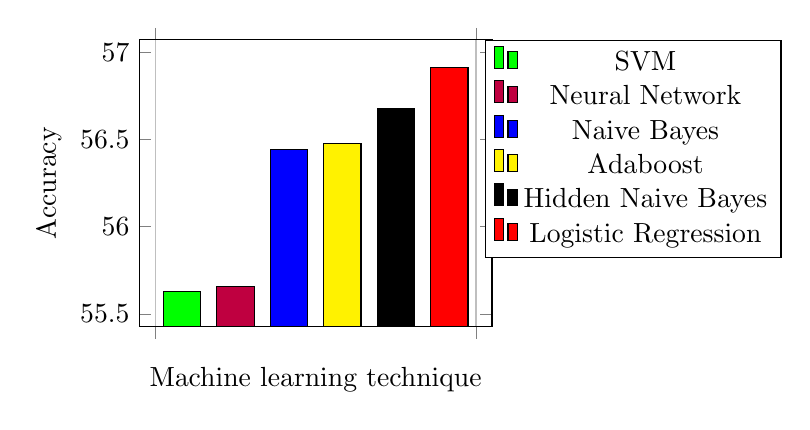
\begin{tikzpicture}
    \begin{axis}[
      %x tick label style={/pgf/number format/1000 sep=},
      xticklabel=\empty,
      ylabel=Accuracy,
      xlabel=Machine learning technique,
      enlargelimits=0.05,
      legend style={at={(1.4,1.0)},
        anchor=north,legend columns=1},
      ybar interval=0.7,
      width=.50\textwidth,
      ymin=55.5, ymax=57,
      reverse legend,
      ]
      \addplot[fill=red] coordinates {(1,56.916) 
        (0,2)
      };
      \addplot[fill=black] coordinates {(1,56.6807) 
        (0,56.6807)
      };
      \addplot[fill=yellow] coordinates {(1,56.479) 
        (0,2)
      };
      \addplot[fill=blue] coordinates {(1,56.4454) 
        (0,56.4454)
      };
      \addplot[fill=purple] coordinates {(1,55.6555) 
        (0,0)
      };
      \addplot[fill=green] coordinates {(1,55.63)
        (0,0)
      };
      \legend{Logistic Regression,Hidden Naive Bayes,Adaboost,Naive Bayes,Neural Network,SVM}
    \end{axis} 
  \end{tikzpicture}
  \caption{Test of best machine learning technique}\label{fig:besttech}
\end{figure}

\subsubsection{Feature symmetry test}
In \Cref{sec:representationoffeatures} we represented four different ways to capture the symmetry of the chosen champions, in this section we are going to test these representations and measure their accuracy. The test was done on an increasing number of matches with all the different methods to check how they hold up with much data. The result, shown in \Cref{fig:feat-rep}, indicates that method 1 and 4 are very close, but binary being slightly above ternary majority of the time, which is the reason for us choosing binary. 

\begin{figure}[!htb]
  \centering
  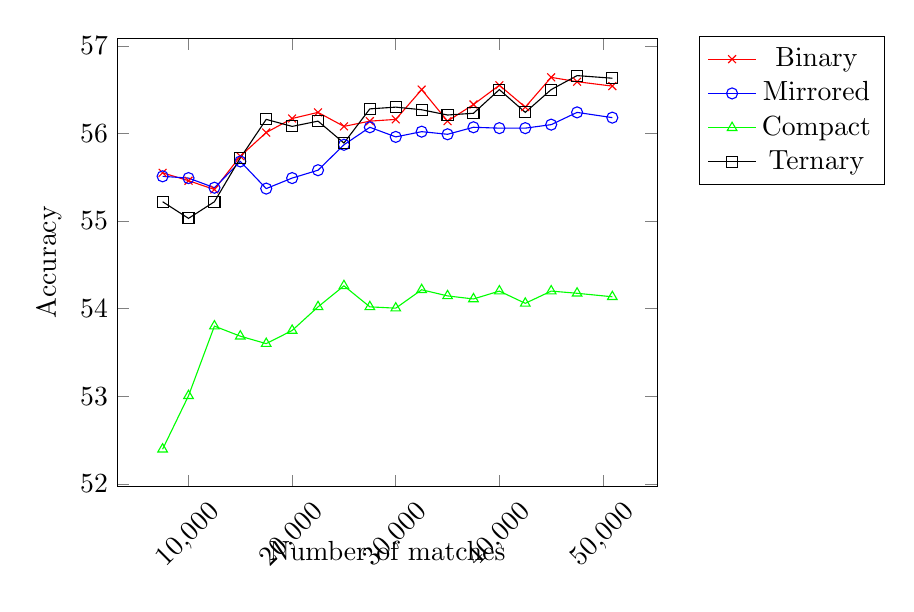
\begin{tikzpicture}[] 
    \begin{axis}[
      xlabel=Number of matches, 
      ylabel=Accuracy,
      xtick={10000,20000,30000,40000,50000},
      xticklabel style={rotate=45,anchor=near xticklabel},
      scaled x ticks=false,
      x label style={at={(axis description cs:0.5,-0.1)},anchor=north},
      legend style={at={(1.25,1.005)},
        anchor=north,legend columns=1},] 
      \addplot[color=red,mark=x] coordinates { 
        (7500, 55.55)
        (10000, 55.46)
        (12500, 55.36)
        (15000, 55.74)
        (17500, 56.01)
        (20000, 56.17)
        (22500, 56.24)
        (25000, 56.08)
        (27500, 56.14)
        (30000, 56.16)
        (32500, 56.50)
        (35000, 56.14)
        (37500, 56.33)
        (40000, 56.55)
        (42500, 56.30)
        (45000, 56.64)
        (47500, 56.59)
        (50901, 56.54)
      };
      \addplot[color=blue,mark=o] coordinates { 
        (7500, 55.51)  
        (10000, 55.49)
        (12500, 55.38)
        (15000, 55.68)
        (17500, 55.37)
        (20000, 55.49)
        (22500, 55.58)
        (25000, 55.87)
        (27500, 56.07)
        (30000, 55.96)
        (32500, 56.02)
        (35000, 55.99)
        (37500, 56.07)
        (40000, 56.06)
        (42500, 56.06)
        (45000, 56.10)
        (47500, 56.24)
        (50901, 56.18)
      };
      \addplot[color=green,mark=triangle] coordinates { 
        (7500, 52.395)  
        (10000, 53.005)
        (12500, 53.80)
        (15000, 53.685)
        (17500, 53.60)
        (20000, 53.75)
        (22500, 54.02)
        (25000, 54.26)
        (27500, 54.02)
        (30000, 54.005)
        (32500, 54.215)
        (35000, 54.145)
        (37500, 54.11)
        (40000, 54.20)
        (42500, 54.06)
        (45000, 54.20)
        (47500, 54.175)
        (50901, 54.135)
      };
      \addplot[color=black,mark=square] coordinates {
        (7500, 55.22)  
        (10000, 55.03)
        (12500, 55.22)
        (15000, 55.72)
        (17500, 56.16)
        (20000, 56.08)
        (22500, 56.14)
        (25000, 55.89)
        (27500, 56.28)
        (30000, 56.30)
        (32500, 56.27)
        (35000, 56.21)
        (37500, 56.23)        
        (40000, 56.50)
        (42500, 56.24)
        (45000, 56.50)
        (47500, 56.66)
        (50901, 56.63)
      };
      \legend{Binary, Mirrored, Compact, Ternary}
    \end{axis} 
  \end{tikzpicture}
  \caption{Test for representation of features}\label{fig:feat-rep}
\end{figure}

\begin{figure}[!htb]
  \centering
  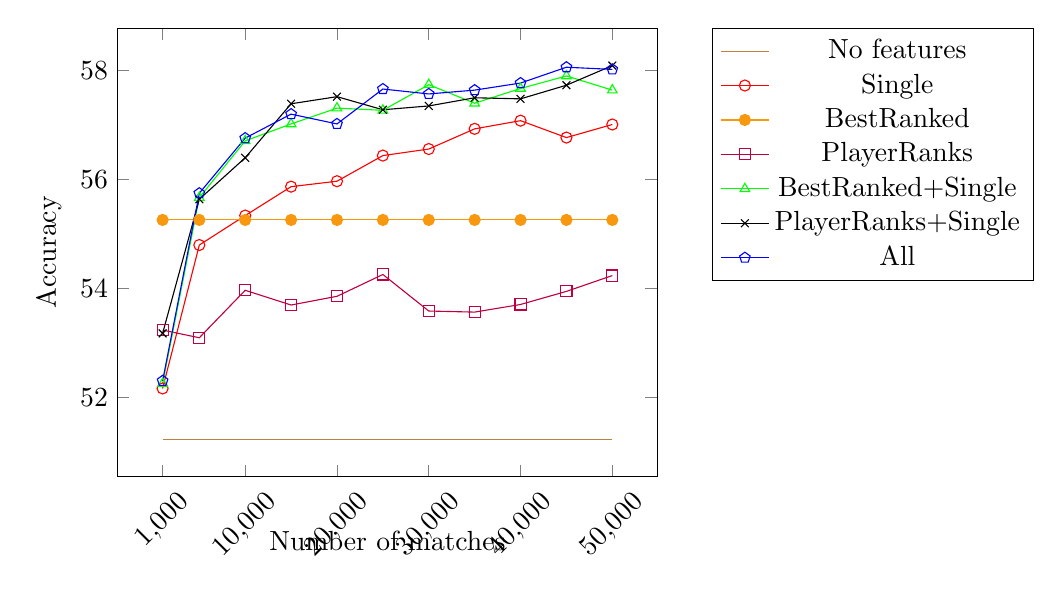
\begin{tikzpicture}[] 
    \begin{axis}[
      xlabel=Number of matches, 
      ylabel=Accuracy,
      xtick={1000,10000,20000,30000,40000,50000},
      xticklabel style={rotate=45,anchor=near xticklabel},
      scaled x ticks=false,
      x label style={at={(axis description cs:0.5,-0.1)},anchor=north},
      legend style={at={(1.4,1.001)},
        anchor=north,legend columns=1},] 
      \addplot[color=brown] coordinates { 
        (1000,51.24)
        (5000,51.24)
        (10000,51.24)
        (15000,51.24)
        (20000,51.24)
        (25000,51.24)
        (30000,51.24)
        (35000,51.24)
        (40000,51.24)
        (45000,51.24)
        (50000,51.24)
      };
      \addplot[color=red,mark=o] coordinates { 
        (1000,52.17)
        (5000,54.8)
        (10000,55.34)
        (15000,55.87)
        (20000,55.97)
        (25000,56.44)
        (30000,56.56)
        (35000,56.93)
        (40000,57.08)
        (45000,56.77)
        (50000,57.01)
      };
      \addplot[color=YellowOrange,mark=*] coordinates { 
        (1000,55.26)
        (5000,55.26)
        (10000,55.26)
        (15000,55.26)
        (20000,55.26)
        (25000,55.26)
        (30000,55.26)
        (35000,55.26)
        (40000,55.26)
        (45000,55.26)
        (50000,55.26)
      };
      \addplot[color=purple,mark=square] coordinates { 
        (1000,53.24)
        (5000,53.1)
        (10000,53.97)
        (15000,53.7)
        (20000,53.86)
        (25000,54.26)
        (30000,53.59)
        (35000,53.57)
        (40000,53.71)
        (45000,53.95)
        (50000,54.24)
      };
      \addplot[color=green,mark=triangle] coordinates { 
        (1000,52.26)
        (5000,55.67)
        (10000,56.71)
        (15000,57.02)
        (20000,57.31)
        (25000,57.27)
        (30000,57.74)
        (35000,57.4)
        (40000,57.67)
        (45000,57.9)
        (50000,57.64)
      };
      \addplot[color=black,mark=x] coordinates { 
        (1000,53.18)
        (5000,55.64)
        (10000,56.4)
        (15000,57.39)
        (20000,57.52)
        (25000,57.28)
        (30000,57.35)
        (35000,57.5)
        (40000,57.48)
        (45000,57.73)
        (50000,58.09)
      };
      \addplot[color=blue,mark=pentagon] coordinates { 
        (1000,52.31)
        (5000,55.75)
        (10000,56.76)
        (15000,57.2)
        (20000,57.02)
        (25000,57.66)
        (30000,57.57)
        (35000,57.64)
        (40000,57.77)
        (45000,58.06)
        (50000,58.02)
      };
      \legend{No features,Single,BestRanked,PlayerRanks,BestRanked+Single,PlayerRanks+Single,All}
    \end{axis} 
  \end{tikzpicture}
  \caption{Accuracy of features}\label{fig:best-feat}
\end{figure}